\documentclass[12pt, fullpage,letterpaper]{article}

\usepackage[margin=1in]{geometry}
\usepackage{amsmath}
\usepackage{listings}
\usepackage{graphicx}
\usepackage{float}
\usepackage{placeins}

\title{Automated Abduction of Differential Equations using Physics Informed Neural Networks}
\author{Roman Amici}

\begin{document}

\maketitle

\section{Introduction}

This report will describe a series of experiments performed in an attempt to infer the form of an underlying differential equation from data using a physics informed neural network (PINN). We were mostly unsuccessful in this endeavor.

\section{Motivation}

The differential loss term in a physics informed neural network can be though of as a general regularization term. That is, when training a PINN on empirical data thought to be generated by a particular differential equation, adding in the differential constraint will reduce overfitting and thus improve generalization. Even without noise, we expect the PINN to perform better. Since neural networks are constructed out of smooth functions, if a given point, $x$ has differential error $O(\epsilon)$, it is likely that nearby points will also have error $O(\epsilon)$ as well.

One could attempt to infer the form of the correct differential by training PINNs regularized by a set of differential equations picked from a library of hypotheses, and choosing the hypothesis which produced the lowest validation error-- provided, of course, that the correct solution was in the library and provided the correct solution does, indeed, dominate all other candidate equations.

The bulk of our investigation was performed on the Burgers Equation on $x \in {-1,1}, t \in {0,1}$ with $u = 0$ for $x = \pm 1$ and $u = \text{sin}(\pi x)$ for $t=0$. The coefficient in front of the diffusion term was $\nu=0.01/\pi$ which produces a shockwave at around $t=0.5$. This setup and architecture was taken from the appendix of the original PINNs paper (Raissi 2018).

\section{Initial Experiments}

In virtually all setups that I can think of, if one doesn't know the form of the differential equation, they also don't know the parameters of that equation either. In the PINN setup, it is possible to jointly infer the parameters and the solution using backpropagation. As a proof of concept, however, we began by assuming that the parameters for the diffusion term, $u_{xx}$ was known and that all other parameters were $1$. 

This makes a bit more sense in context as we were initially interested in whether an incomplete equation might might be helpful for regularization. The Burgers equation is typically used to describe viscous fluids and has form
\[
    \frac{\partial u}{\partial t} + u \frac{\partial u}{\partial x} = \nu \frac{\partial^2}{\partial x^2}
\]
It seems sensible to ask whether regularization based on non-viscid fluids which has the form
\[
    \frac{\partial u}{\partial t} + u \frac{\partial u}{\partial x} = 0
\]
might improve validation accuracy especially if $\nu$ is small.

\begin{figure}[!htb]
    \centering
    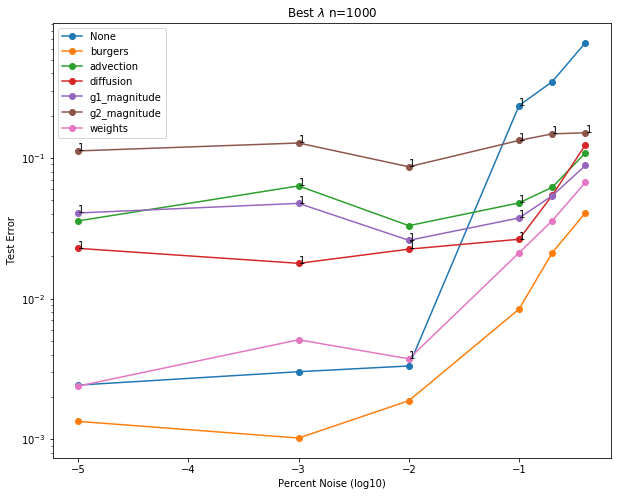
\includegraphics[width=\textwidth]{reduced-scaling-1000}
    \caption{Neural network regularized with the true equation (burgers) dominate the other forms of regularization. Best value of regularization $\lambda$ was chosen for display. For Burgers, this was typically $\lambda = 1$.}
    \label{fig:reduced-scaling}
\end{figure}

As Figure \ref{fig:reduced-scaling} shows, using the pure advection and diffusion equations, results in a worse fit. It appears that burgers does dominate all other forms of regularization including advection and diffusion. These results generalized when $\nu$ had to be inferred and noise was also added to the evaluation set (see Figure \ref{fig:reduced-noisy-eval}).

\begin{figure}[!htb]
    \centering
    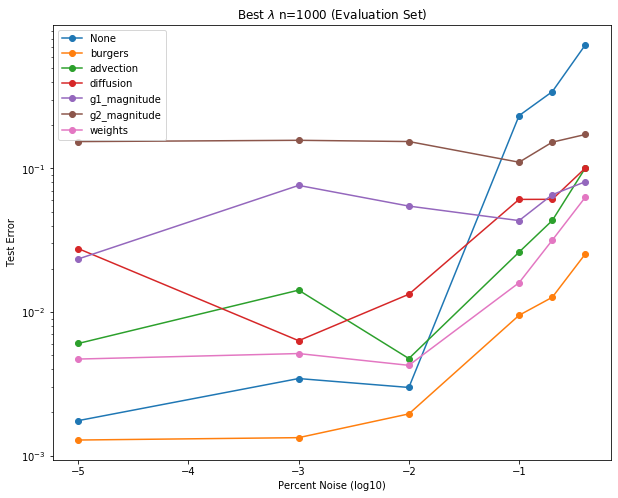
\includegraphics[width=\textwidth]{reduced-scaling-1000-eval}
    \caption{Results with $\nu$ inferred and evaluated on a noisy evaluation set.}
    \label{fig:reduced-noisy-eval}
\end{figure}

\section{Automated Abduction with Known Parameters }

We attempted to see if this would persist in the presence of additional ``nuisance'' terms in the search space. The size of the search space, however, grows like $2^{|L|}$ where $|L|$ is the size of the term library. It would thus be impossible to try every combination of terms. It was thus necessary to find a better way to cover the search space. This can be cast as a black-box optimization problem. We want to find a global optima in the error space. However, evaluating an configuration requires training a full model and is thus quite expensive. Instead we construct a surrogate model of the error which we use to suggest new configurations to search. 

Our initial experiments used Bayesian Optimization with a Gaussian Process as a surrogate. However, GP's are necessarily continuos whereas the presence and absence of term is discrete. It was hoped that relaxing the parameters would be sufficient. However, this was not the case. The correct solution was found in a number of iterations that was no better than brute-force search. Indeed, it was sometimes worse since the Bayesian Optimization process would often repeatedly resample the same high-performing configuration due to the relaxation.

Instead we switched to SMAC which uses a random forest technique to handle discrete variables. This was more successful. In the small search space of size 512, we were able to find the correct solution 100\% of the time within 100 iterations. In the large configuration of size 4096 we were able to achieve find the solution 84\% of the time after searching for 500 iterations. During this tests, we reported no ``false negatives'', that is, times where the correct configuration was tried as a candidate by the surrogate, but rejected in favor of a better version.

To reiterate, this was done in the setting where we assumed that we already knew the correct value of $\nu$, and all other parameters were fixed at 1. When this assumption was relaxed, the results were quite bad. The correct solution was never recovered. Additionally, the results were rife with false negatives. It frequently chose other equations despite trying the correct equation as a candidate. These results appear to kill any hope of using this technique to do black box abduction of differential equations.

\section{Automated Abduction with Inferred Parameters}

What appears to account for all of the false negatives? First, its worth pointing out that when regularized on the correct differential equation with the exact correct parameter, the results are still superior to the false positive equations. The correct equation with correct parameters has RSME on the around 0.008. The incorrect solutions which it chose have error between 0.02 and 0.04. However, the correct equation with inferred parameters appears to have error in this range as well. 

\begin{figure}[!htb]
    \centering
    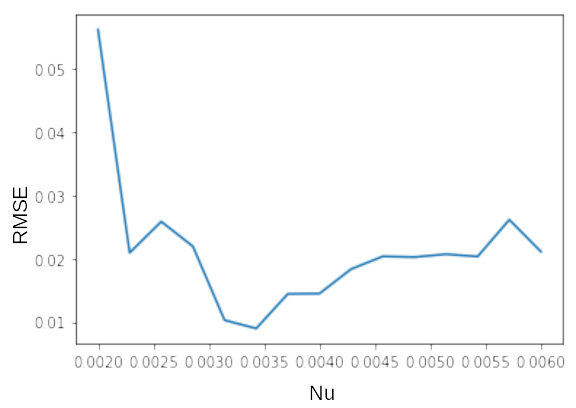
\includegraphics[width=\textwidth]{nu-scaling-labeled}
    \caption{Error for a PINN using a variety of (static) values of $\nu$}
    \label{fig:burgers-nu-sensitivity}
\end{figure}

Some of this behavior can be explained by Figure \ref{fig:burgers-nu-sensitivity}. The effect of the PINN regularization is sensitive to the value of $\nu$. The inferred parameter must be able to get very close to the correct value to see a large jump in resolution. Burgers, after all, is a non-linear equation, and thus small changes in the value of $\nu$ can lead to large changes in the solution.

Why, do the other equations do so well? Its not obvious that they do much better than generic regularization like $L^2$ though still a bit better. I conjecture that it can partially be explained ease with which it can make certain parameters small effectively negating their impact. It might also have to do with the fact that spurious derivative terms can approximate other terms via taylor expansion and thus simply adding more terms can partially fill in for other, missing terms.


\end{document}